\section{Definiciones Básicas}

\begin{itemize}
    \item Sistema Termodinámico:
    Un agrupamiento de partículas comprendido en una frontera o
    superficie $S$.
    \item Contacto Térmico entre dos sistemas:
    Es el intercambio de energía entre dos sistemas.
    \item Equilibrio Térmico en un sistema:
    Se da cuando la temperatura de cualquier subsitema, contenido en el
    ``original'', es la misma y se mantiene por un tiempo
    representativo.
    \item Equilibrio Térmico entre dos sistemas:
    Se da cuando los dos sistemas se encuentran a la misma temperatura.
\end{itemize}

\section{Leyes cero, uno y dos de la Termodinámica}

\subsection{Ley 0}
Sean $A$, $B$ y $C$ sistemas termodinámicos. Si el sistema $C$ se
encuentra en contacto térmico y en equilibrio con los sistemas $A$ y
con $B$. Entonces $A$ se encuentra en equilibrio térmico con $B$.

\begin{center}
    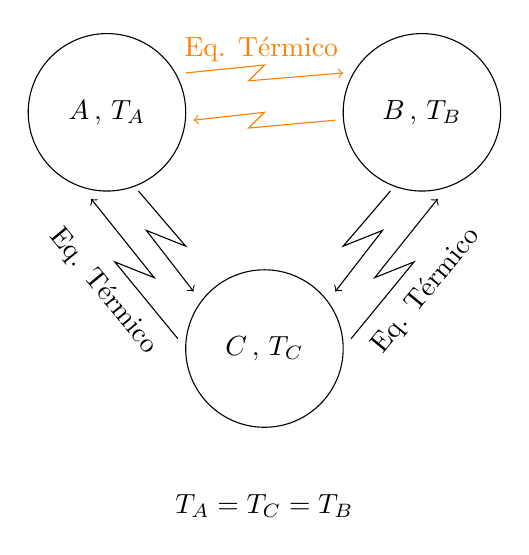
\begin{tikzpicture}
        % ~~~~ Sistemas ~~~~ %
        \draw (0,0) circle (1)
            node {$A\,,\,T_A$};
        \draw (4,0) circle (1)
            node {$B\,,\,T_B$};
        \draw (2,-3) circle (1)
            node {$C\,,\,T_C$};
        
        % ~~~~ Rayos/Rep.Energia ~~~~ %
        \draw[orange, ->] (1, 0.5) -- (2, 0.6) -- (1.8, 0.4) -- (3, 0.5)
            node[midway,xshift=-12.5, yshift=10] {Eq. Térmico};
        \draw[orange, ->] (2.9,-0.1) -- (1.8,-0.2) -- (2,0) -- (1.1,-0.1);

        \draw[ -> ] (0.4,-1) -- (1,-1.7) -- (0.5, -1.5) --  (1.1,-2.275);
        \draw[ <- ] (-0.2,-1.1) -- (0.6,-2.1) -- (0.1, -1.9) --  (0.9,-2.875)
            node[midway,xshift=-12.5,yshift=-10, sloped] {Eq. Térmico};

        \draw[ -> ] (4-0.4,-1) -- (4-1,-1.7) -- (4-0.5, -1.5) --  (4-1.1,-2.275);
        \draw[ <- ] (4+0.2,-1.1) -- (4-0.6,-2.1) -- (4-0.1, -1.9) --  (4-0.9,-2.875)
            node[midway,xshift=12.5,yshift=-10, sloped] {Eq. Térmico};

        % ~~~~ Resultado/Ley ~~~~ %
        \draw (2,-5) node {$T_A = T_C =T_B$};
    \end{tikzpicture}
\end{center}

\subsection{Primera Ley}
La energía del universo ($U$) se conserva. Esto es, en cualquier par de
instantes de tiempo, la energía debe ser igual.

Sea $A$ un subsistema del universo con una energía asosiada $U_A$; y
sea $U_E$ la energía asociada al resto del universo. En un intervalo de
tiempo, la energía inicial debe ser igual a la energía final:
$U = U_E + U_A$ . Si se produce un intercambio de energía entre los dos
sistemas mencionados para el momento final del intervalo de tiempo, se
tiene entonces que:
\[
    \begin{derivation}
            \res{U_{\text{final}} = U_{\text{inicial}}}\\
        \equiv\\
            \res{ U_E + \Delta U_E + U_A + \Delta U_A = U_E + U_A}\\
        \equiv\\
            \res{ \Delta U_E = -\Delta U_A}
    \end{derivation}
\]

\subsection{Segunda Ley}
La energía de tipo calor ($Q$) siempre fluye naturalmente de los sistemas con
mayor temperatura a los de menor temperatura.

\begin{center}
    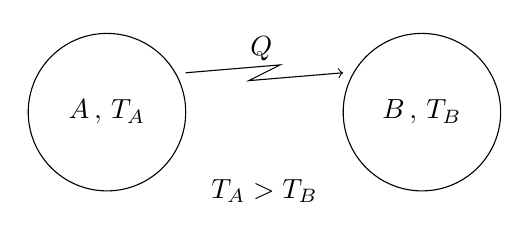
\begin{tikzpicture}
        % ~~~~ Sistemas ~~~~ %
        \draw (0,0) circle (1) node {$A\,,\,T_A$};
        \draw (4,0) circle (1) node {$B\,,\,T_B$};

        % ~~~~ Energía ~~~~ %
        \draw[ -> ] (1,0.5) -- (2.2,0.6) -- (1.8,0.4) -- (3,0.5)
            node[midway,xshift=-12.5,yshift=10] {$Q$};

        % ~~~~ Hipótesis ~~~~ %
        \draw (2,-1) node {$T_A > T_B$};
    \end{tikzpicture}
\end{center}